% Figure: the tapped shape column — jets by subtraction. Referenced from §12's
% prop:gamma-jets. Pure TikZ; the plan table's "tapped cascade" figure. Shown for γ = 3,
% n up to 2.

\begin{figure}[t]
\centering
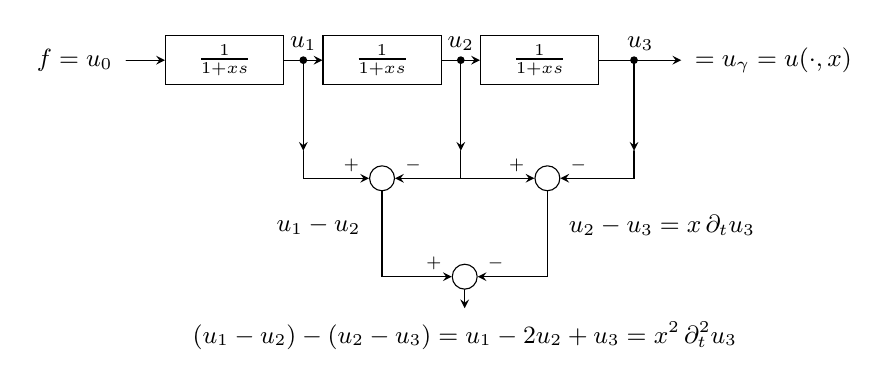
\begin{tikzpicture}[every node/.style={font=\small}, line cap=round, >=stealth,
  sect/.style={draw, minimum width=1.5cm, minimum height=0.62cm, inner sep=2pt},
  sum/.style={draw, circle, inner sep=1.0pt}]

% the shape column: three identical leaky integrators at time constant x
\node[anchor=east] at (-0.2,0) {$f = u_0$};
\node[sect] (s1) at (1.1,0) {$\frac{1}{1+xs}$};
\node[sect] (s2) at (3.1,0) {$\frac{1}{1+xs}$};
\node[sect] (s3) at (5.1,0) {$\frac{1}{1+xs}$};
\draw[->] (-0.15,0) -- (s1.west);
\draw[->] (s1) -- node[above] {$u_1$} (s2);
\draw[->] (s2) -- node[above] {$u_2$} (s3);
\draw[->] (s3.east) -- node[above] {$u_3$} (6.9,0);
\node[anchor=west] at (6.95,0) {$= u_\gamma = u(\cdot, x)$};

% taps down to the subtraction row
\foreach \xx in {2.1, 4.1, 6.3} \fill (\xx,0) circle (1.4pt);
\draw[->] (2.1,0) -- (2.1,-1.15);
\draw[->] (4.1,0) -- (4.1,-1.15);
\draw[->] (6.3,0) -- (6.3,-1.15);

% first differences: adjacent taps, minuend marked +, subtrahend marked -
% (redrawn 2026-08-31, author review: the second difference was drawn as a "+" node
% fed by u_1, u_2, u_2 - u_3, whose true signs are (+,-,-); it is now the difference
% of the two first differences, every input signed)
\node[sum, minimum size=9pt] (dA) at (3.1,-1.5) {};
\draw[->] (2.1,-1.15) -- (2.1,-1.5) -- (dA.west);
\draw[->] (4.1,-1.15) -- (4.1,-1.5) -- (dA.east);
\node[inner sep=1pt, anchor=south east] at (2.85,-1.46) {$\scriptstyle +$};
\node[inner sep=1pt, anchor=south west] at (3.35,-1.46) {$\scriptstyle -$};
\node[sum, minimum size=9pt] (dB) at (5.2,-1.5) {};
\draw[->] (4.1,-1.5) -- (dB.west);
\draw[->] (6.3,-1.15) -- (6.3,-1.5) -- (dB.east);
\node[inner sep=1pt, anchor=south east] at (4.95,-1.46) {$\scriptstyle +$};
\node[inner sep=1pt, anchor=south west] at (5.45,-1.46) {$\scriptstyle -$};
\node[anchor=east] at (2.95,-2.1) {$u_1 - u_2$};
\node[anchor=west] at (5.35,-2.1) {$u_2 - u_3 = x\,\partial_t u_3$};

% second difference: difference of the first differences
\node[sum, minimum size=9pt] (d2) at (4.15,-2.75) {};
\draw[->] (dA.south) -- (3.1,-2.75) -- (d2.west);
\draw[->] (dB.south) -- (5.2,-2.75) -- (d2.east);
\node[inner sep=1pt, anchor=south east] at (3.9,-2.71) {$\scriptstyle +$};
\node[inner sep=1pt, anchor=south west] at (4.4,-2.71) {$\scriptstyle -$};
\draw[->] (d2.south) -- (4.15,-3.15);
\node[anchor=north] at (4.15,-3.2) {$(u_1 - u_2) - (u_2 - u_3) = u_1 - 2u_2 + u_3 = x^2\,\partial_t^2 u_3$};

\end{tikzpicture}
\caption{Jets by subtraction along the shape column ($\gamma = 3$). The column of
$\gamma$ identical leaky integrators at time constant $x$ --- the pure-pole cascade from
scale zero, the gamma memory of \sscite{devries1992gamma} --- carries the fields
$u_0, \dots, u_\gamma$ of increasing shape as coexisting states. The scale-normalized jet
at scale $x$ is read off the taps by binomial-weighted subtraction,
$x^n\partial_t^n u_\gamma = \sum_j (-1)^{n-j}\binom{n}{j}u_{\gamma-j}$, realized as
iterated differences of adjacent taps
(Proposition~\ref{prop:gamma-jets}): no temporal differencing, and no second memory,
anywhere in the architecture.}
\label{fig:jet-taps}
\end{figure}
